\chapter{Introduction}

Graph theory is a branch of discrete mathematics concerned with the study of structures composed of \textbf{vertices} (nodes) and \textbf{edges} (connections). Although originating with Euler’s 1736 solution to the Königsberg Bridge Problem \cite{euler1736}, it has evolved into a major mathematical discipline with extensive applications in modern computer science, data science, network analysis and artificial intelligence.

\section{Why Graph Theory Matters in Data Science}

Many datasets today are relational rather than tabular.  
Examples include:
\begin{itemize}
	\item Social networks — users connected via friendships.
	\item Web graphs — websites connected by hyperlinks.
	\item Transportation systems — cities connected by routes.
	\item Biological networks — proteins interacting with one another.
\end{itemize}

Traditional statistical methods often fail to capture this relational structure. Graph theory provides:
\begin{itemize}
	\item Mathematical tools for modeling connected systems.
	\item Algorithms for efficient search, traversal and pattern discovery.
	\item Foundations for emerging fields such as Graph Neural Networks (GNNs) \cite{kipf2017semi}.
\end{itemize}

\section{Basic Graph Concept Illustration}

Figure~\ref{fig:simple_graph} shows a basic undirected graph.

\begin{figure}[H]
	\centering
	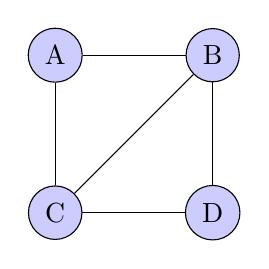
\begin{tikzpicture}[node distance=2cm, every node/.style={circle, draw, fill=blue!20}]
		\node (A) {A};
		\node (B) [right of=A] {B};
		\node (C) [below of=A] {C};
		\node (D) [below of=B] {D};
		
		\draw (A)--(B);
		\draw (A)--(C);
		\draw (B)--(C);
		\draw (B)--(D);
		\draw (C)--(D);
	\end{tikzpicture}
	\caption{A sample undirected graph with four vertices.}
	\label{fig:simple_graph}
\end{figure}

\section{Structure of This Report}

This report is divided into five chapters:

\begin{itemize}
	\item \textbf{Chapter 1}: Introduction to graph theory and its relevance.
	\item \textbf{Chapter 2}: Formal mathematical foundations and graph structures.
	\item \textbf{Chapter 3}: Classical graph algorithms used in data science.
	\item \textbf{Chapter 4}: Advanced topics including spectral graph theory and GNNs.
	\item \textbf{Chapter 5}: Conclusions and implications for data-driven applications.
\end{itemize}